\section{Homework 2}
\subsection{Exercise 2.28}
A matrix is positive semi-definite if we define two matrices symmetric $A$ and $Q$, such that $Q(\textbf{x}) = \textbf{x}^T A \textbf{x} $, $Q$ and $A$ are positive semidefinite if $Q(\textbf{x}) \geq 0$ for all $\textbf{x}$.
\\
In other words, for a matrix $A$ to be positive semidefinite, these two conditions must be satisfied:
\begin{itemize}
  \item $A$ is symmetric
  \item $x^T A x \geq 0$ for all $x$
\end{itemize}
The second condition can be broadened to multiple equivalent definitions:
\begin{itemize}
  \item $x^T A x \geq 0$ for all $x$
  \item All eigenvalues are non-negative
  \item There exists a matrix $B$ s.t. $B^TB = A$
  \item All principal minors are non-negative
\end{itemize}
\subsubsection{n=1}
For $n = 1 $, the cone is defined by the inequality $x_1 \geq 0 $
\subsubsection{n=2}
$x_1x_3 - x_2^2 \geq 0 $ and $x_1,x_3 \geq 0$
\subsubsection{n=3}
All principal minors must be non-negative, so blocking off each row and column of the matrix.
\\ \\
Diagonals: $x_1,x_4,x_6 \geq 0$
\\ \\ 
Full matrix determinant: $x_1 (x_4 x_6 - x_5^2) - x_2 (x_2 x_6 - x_3 x_5) + x_3(x_2 x_5 - x_3 x_4) \geq 0$
2x2 determinants: $x_4 x_6 - x_5^2 \geq 0$, $ x_1 x_6 - x_3^2 \geq 0$ $ x_1 x_4 - x_2^2 \geq 0 $ 
\subsection{Exercise 2.33}
\subsubsection{part a}
A convex cone $K \subseteq \mathbb{R}^n$ is a proper cone if
\begin{itemize}
  \item K is closed (contains its boundary)
  \item K is solid (nonempty interior)
  \item K is pointed (contains no line)
\end{itemize}
For this problem, we must show that the monotone non-negative cone defined as 
\begin{equation}
  K_{m+} = \{ \textbf{x} \in \mathbb{R}^n | x_1 \geq x_2 \geq \dots \geq x_n \geq 0 \}
\end{equation}
is a proper cone.
\\ \\
Proving the first, where $K_{m+}$ is closed and contains its boundary, we first find the boundary of $K_{m+}$. The boundaries are the two vectors in the direction of 
\begin{align}
  \begin{bmatrix}
     1 \\
     0 \\
     \vdots \\
     0
  \end{bmatrix},
  \begin{bmatrix}
    1 \\
    1 \\
    \vdots \\
    1
  \end{bmatrix}
\end{align}
With magnitude $x_1$. These boundaries clearly satisfy the $\geq$ requirements of the set. If one of the conditions was a strict equality, then the convex cone would be open.
\\ \\
Proving the second, since all vectors are contained in between the boundaries, the set is solid.
\\ \\ 
Proving the third, because of the $\geq 0$ requirement, the $\textbf{x}\in \mathbb{R}^n$ of the set also have the $\textbf{x} \succeq 0 $ applicable. Therefore the cone is pointed.
\begin{figure}[htbp]
  \centerline{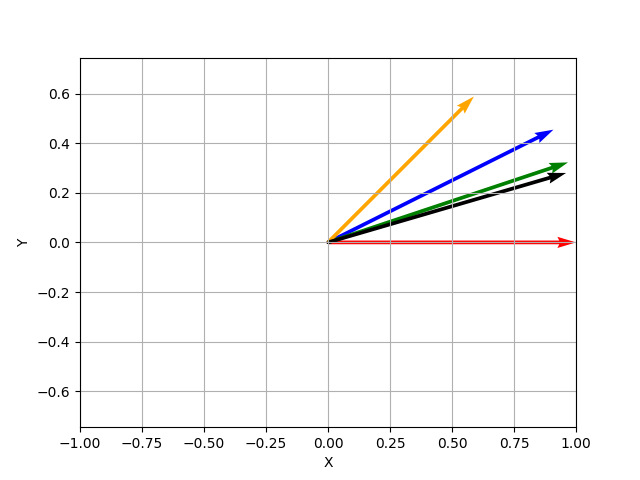
\includegraphics[width=0.50\textwidth]{hw2/images/exercise233cone.png}}
  \caption{Image of a monotone non-negative cone in $\mathbb{R}^2$}
  \label{fig:exercise233cone}
\end{figure}
\subsubsection{part b}
Finding the dual cone $K_{m+}^*$. A dual cone is defined as 
\begin{equation}
  K^* = \{ y | x^T y \geq 0 \text{ for all } x\in K \}
\end{equation}
\begin{gather}
  x^T y \\
  = \sum_{i=1}^n x_i y_i \\
  = (x_1 - x_2)y_1 + (x_2 -x_3)(y_1+y_2) + \dots + (x_{n-1} - x_n)(y_1+\dots + y_n-1) + x_n(y_1+\dots + y_n)
\end{gather}
Since each term of $y$ is getting multiplied by $x_i - x_{i+1}$, and $x_i \geq x_{i+1}$, each $y$ term is getting multiplied by a non-negative $x$ term, so if we want $x^T y \geq 0$ for all x, then we will need in the worst case scenario, for each one of the $y$ terms to be positive.
\begin{equation}
  y_1 \geq 0, y_1 + y_2 \geq 0, y_1 + y_2 + y_3 \geq 0, \dots, \sum_{i=1}^{n} y_i \geq 0
\end{equation}
These conditions are all satisfied when $y_n \geq y_{n-1} \geq \dots \geq y_2 \geq y_1 \geq 0$. Therefore, the dual cone is 
\begin{equation}
  K^* = \{ y \in \mathbb{R}^n | y_n \geq y_{n-1} \geq \dots \geq y_2 \geq y_1 \geq 0\}
\end{equation}
\subsection{Exercise 3.2}

\subsection{Exercise 3.5}

\subsection{Exercise 3.6}

\subsection{Exercise 3.15}

\subsection{Exercise 3.16}

\subsection{Exercise 3.18}

\subsection{Exercise 3.24}

\subsection{Exercise 3.36}

